\documentclass[11pt,compress,t,notes=noshow, xcolor=table]{beamer}
\usepackage[]{graphicx}\usepackage[]{color}
% maxwidth is the original width if it is less than linewidth
% otherwise use linewidth (to make sure the graphics do not exceed the margin)
\makeatletter
\def\maxwidth{ %
  \ifdim\Gin@nat@width>\linewidth
    \linewidth
  \else
    \Gin@nat@width
  \fi
}
\makeatother

\definecolor{fgcolor}{rgb}{0.345, 0.345, 0.345}
\newcommand{\hlnum}[1]{\textcolor[rgb]{0.686,0.059,0.569}{#1}}%
\newcommand{\hlstr}[1]{\textcolor[rgb]{0.192,0.494,0.8}{#1}}%
\newcommand{\hlcom}[1]{\textcolor[rgb]{0.678,0.584,0.686}{\textit{#1}}}%
\newcommand{\hlopt}[1]{\textcolor[rgb]{0,0,0}{#1}}%
\newcommand{\hlstd}[1]{\textcolor[rgb]{0.345,0.345,0.345}{#1}}%
\newcommand{\hlkwa}[1]{\textcolor[rgb]{0.161,0.373,0.58}{\textbf{#1}}}%
\newcommand{\hlkwb}[1]{\textcolor[rgb]{0.69,0.353,0.396}{#1}}%
\newcommand{\hlkwc}[1]{\textcolor[rgb]{0.333,0.667,0.333}{#1}}%
\newcommand{\hlkwd}[1]{\textcolor[rgb]{0.737,0.353,0.396}{\textbf{#1}}}%
\let\hlipl\hlkwb

\usepackage{framed}
\makeatletter
\newenvironment{kframe}{%
 \def\at@end@of@kframe{}%
 \ifinner\ifhmode%
  \def\at@end@of@kframe{\end{minipage}}%
  \begin{minipage}{\columnwidth}%
 \fi\fi%
 \def\FrameCommand##1{\hskip\@totalleftmargin \hskip-\fboxsep
 \colorbox{shadecolor}{##1}\hskip-\fboxsep
     % There is no \\@totalrightmargin, so:
     \hskip-\linewidth \hskip-\@totalleftmargin \hskip\columnwidth}%
 \MakeFramed {\advance\hsize-\width
   \@totalleftmargin\z@ \linewidth\hsize
   \@setminipage}}%
 {\par\unskip\endMakeFramed%
 \at@end@of@kframe}
\makeatother

\definecolor{shadecolor}{rgb}{.97, .97, .97}
\definecolor{messagecolor}{rgb}{0, 0, 0}
\definecolor{warningcolor}{rgb}{1, 0, 1}
\definecolor{errorcolor}{rgb}{1, 0, 0}
\newenvironment{knitrout}{}{} % an empty environment to be redefined in TeX

\usepackage{alltt}
\newcommand{\SweaveOpts}[1]{}  % do not interfere with LaTeX
\newcommand{\SweaveInput}[1]{} % because they are not real TeX commands
\newcommand{\Sexpr}[1]{}       % will only be parsed by R



\usepackage[english]{babel}
\usepackage[utf8]{inputenc}

\usepackage{dsfont}
\usepackage{verbatim}
\usepackage{amsmath}
\usepackage{amsfonts}
\usepackage{bm}
\usepackage{csquotes}
\usepackage{multirow}
\usepackage{longtable}
\usepackage{booktabs}
\usepackage{enumerate}
\usepackage[absolute,overlay]{textpos}
\usepackage{psfrag}
\usepackage{algorithm}
\usepackage{algpseudocode}
\usepackage{eqnarray}
\usepackage{arydshln}
\usepackage{tabularx}
\usepackage{placeins}
\usepackage{tikz}
\usepackage{setspace}
\usepackage{colortbl}
\usepackage{mathtools}
\usepackage{wrapfig}
\usepackage{bm}
\usetikzlibrary{shapes,arrows,automata,positioning,calc,chains,trees, shadows}
\tikzset{
  %Define standard arrow tip
  >=stealth',
  %Define style for boxes
  punkt/.style={
    rectangle,
    rounded corners,
    draw=black, very thick,
    text width=6.5em,
    minimum height=2em,
    text centered},
  % Define arrow style
  pil/.style={
    ->,
    thick,
    shorten <=2pt,
    shorten >=2pt,}
}
\usepackage{subfig}


% Defines macros and environments
\input{../../style/common.tex}

%\usetheme{lmu-lecture}
\newcommand{\titlefigure}{figure_man/intro-titlefig.jpg}
\newcommand{\learninggoals}{
\item Understand the goal of performance estimation
\item Know the definition of generalization error
\item Understand the difference between outer and inner loss}
\usepackage{../../style/lmu-lecture}

\let\code=\texttt
\let\proglang=\textsf

\setkeys{Gin}{width=0.9\textwidth}

\title{Introduction to Machine Learning}
% \author{Bernd Bischl, Christoph Molnar, Daniel Schalk, Fabian Scheipl}
\institute{\href{https://compstat-lmu.github.io/lecture_i2ml/}{compstat-lmu.github.io/lecture\_i2ml}}
\date{}

\setbeamertemplate{frametitle}{\expandafter\uppercase\expandafter\insertframetitle}


\begin{document}


% This file loads R packages, configures knitr options and sets preamble.Rnw as parent file
% IF YOU MODIFY THIS, PLZ ALSO MODIFY setup.Rmd ACCORDINGLY...


% Defines macros and environments
\input{../../latex-math/basic-math.tex}
\input{../../latex-math/basic-ml.tex}
\input{../../latex-math/ml-automl.tex}
%! includes: basics-learners 

\lecturechapter{Evaluation: Introduction and Remarks}
\lecture{Introduction to Machine Learning}

% ------------------------------------------------------------------------------

\begin{vbframe}{Performance estimation}

\begin{itemize}
  \item After training our model, we are naturally interested in its
  \textbf{performance}.
  \item Recall that supervised learning is about finding the optimal model 
  for our data at hand, given a set of hyperparameters: 
  $$\inducer: \preimageInducerShort \rightarrow \Hspace, \quad (\D, \lambdav)
  \mapsto \fh_{\D, \lambdav}.$$
  \item We obtain $\fh_{\D, \lambdav}$ by means of empirical risk minimization, 
  based on what we will now call \textbf{inner loss}.
  \item However, the inner loss does not tell us anything about the performance 
  of our learner -- after all, we chose our model precisely so it would be 
  loss-minimal on the data we trained it on.
\end{itemize}

\lz
$\rightarrow$ We cannot hope for $\fh_{\D, \lambdav}$ to perform equally well 
on unseen data. \\
$\rightarrow$ Evaluation based on the inner loss would be 
\textbf{optimistically biased}.

\framebreak

\begin{itemize}
  \item We wish to compute the true expected loss of our learner, referred to as
  \textbf{generalization error} or \textbf{outer loss}.
\end{itemize}

\begin{center}
% FIGURE SOURCE: https://docs.google.com/drawings/d/13AH298rMnDL5p0SrBd6VCukC9vg1qyRXGqgMcvuPRc0/edit?usp=sharing
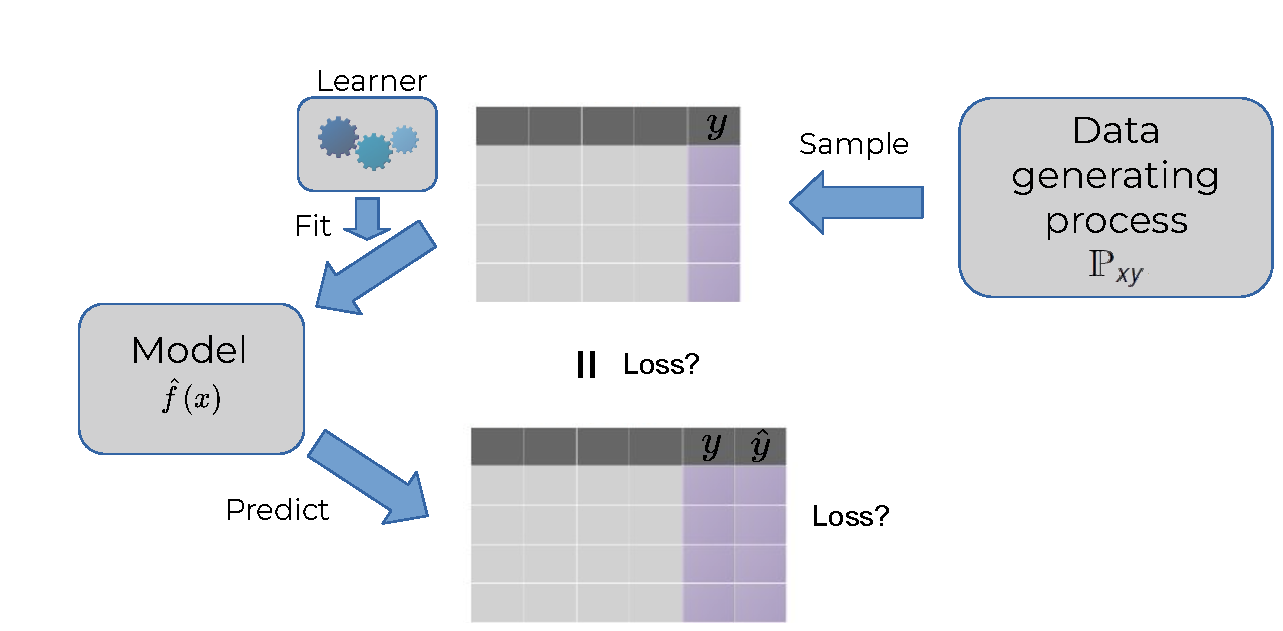
\includegraphics[trim = 0 0 0 30, clip, width=0.7\textwidth]
{figure_man/evaluation-intro-ge.pdf}
\end{center}

\begin{itemize}
  \item In order to estimate performance on previously unseen observations, we 
  need independent \textbf{test data}. 
  \item As such a test set is not always available, we make do with 
  splitting our data at hand into non-overlapping sets $\Dtrain$ and $\Dtest$, 
  with respective sizes $m_{\mathrm{train}} + m_{\mathrm{test}} = n$.
\end{itemize}

\end{vbframe}

% ------------------------------------------------------------------------------

\begin{vbframe}{Set-based performance metrics}

\begin{itemize}
  \item For the outer loss, we introduce a \textbf{set-based metric} $\rho$.
  \item This allows us to use outer losses that are defined on the entire test 
  set rather than point-wise (e.g., the AUC), and potentially differ from the 
  inner loss.
  \item For arbitrary data sets of size $m$ and a prediction matrix 
  $\bm{F} \in \R^{m \times g}$ returned by our model, $\rho$ is defined as:
  $$\rho: \bigcup_{m \in \N} \left( \Yspace^m \times \R^{m \times g} \right) 
  \rightarrow \R, \quad (\yv, \bm{F}) \mapsto \rho(\yv, \bm{F}).$$
  \item We can easily translate this to our usual notion of point-wise loss:
  $$\rho_L(\yv, \bm{F}) = \sum_{i=1}^m L(\yi, \bm{F}^{(i)}).$$
\end{itemize}

\end{vbframe}

% ------------------------------------------------------------------------------

\begin{vbframe}{Generalization error}

\begin{itemize}
  % \item To ease notation, we will represent our train and test sets by index 
  % vectors $J_\mathrm{train} \in \nset^{m_\mathrm{train}}$ and $J_\mathrm{test} 
  % \in \nset^{m_\mathrm{test}}$.
  % \item With this, we can denote the corresponding vector of labels as
  % $\yv_J = \left(y^{(J^{(1)})},\dots, y^{(J^{(m)})} \right) \in \Yspace^m$ and 
  % the matrix of prediction scores as
  % $\bm{F}_{J,f} = \left( f(\xv^{(J^{(1)})}), \dots, f(\xv^{(J^{(m)})}) \right)
  % \in \R^{m\times g}$.
  \item This allows us to define the \textbf{generalization error} as:
  $$\mathrm{GE}(\inducer, \lambdav, m_{\mathrm{train}}, \rho) := 
  \lim_{m_{\mathrm{test}} \rightarrow \infty} \E \left[ \rho \left(
  \yv, \bm{F}_{\Dtest, \inducer(\mathcal{D}_{\mathrm{train}}, \lambdav)} 
  \right)\right].$$
  \item The expectation is taken w.r.t. the unkown distribution $\Pxy$ from 
  which both $\Dtrain$ and $\Dtest$ are sampled independently.
  \item We must therefore estimate the generalization error, based on our 
  train-test split:
  $$\widehat{\mathrm{GE}}_{\Dtrain, \Dtest}(\inducer,
  \lambdav, m_\mathrm{train}, \rho) =
  \rho \left( \yv_{\Dtest}, \bm{F}_{\Dtest, 
  \inducer(\mathcal{D}_{\mathrm{train}}, \lambdav)} \right).$$
  \item In practice, we will not rely on a single split, but use 
  \textbf{resampling} to repeatedly carve out test observations from our data.
\end{itemize}

\end{vbframe}

% ------------------------------------------------------------------------------

\begin{vbframe}{Inner vs outer loss}

\begin{itemize}
  \item Supervised learning thus implies the following dichotomy:
  \begin{itemize}
    \item \textbf{Learning}: minimize inner loss
    \item \textbf{Evaluation}: estimate outer loss
  \end{itemize}
  \item Beyond evaluating a single learner, the outer loss lends itself to
  comparing different types of learners, or learners with varying hyperparameter
  configurations $\lambdav$.
  \lz
  \item Ideally, we have \textbf{inner loss = outer loss}.
  \item This is not always possible -- some special (set-based) metrics for 
  evaluation, such as the AUC, are not applicable as inner loss.
  \item On the other hand, we sometimes wish to use losses that are 
  hard to optimize or do not even specify one directly.
  % , as in:
  % \begin{itemize}
  %   \item Logistic regression: minimization of binomial loss
  %   \item k-NN: no explicit loss minimization
  % \end{itemize}
\end{itemize}

\framebreak

\textbf{Example:} Logistic regression

\begin{itemize}
  \item An intuitive choice would be the share of incorrect predictions.
  \item This leads to the \textbf{mislassification error rate (MCE)}, computing
  the mean over pointwise \textbf{0-1 loss}.
\end{itemize}

\lz

\begin{minipage}{0.6\textwidth}
  \begin{itemize}
    \item 0-1 loss simply assigns a loss of 1 for incorrect predictions and 0
    otherwise: $$\Lhxy = [y \neq \hx]$$
  \end{itemize}
\end{minipage}%
\begin{minipage}{0.4\textwidth}
  \centering
  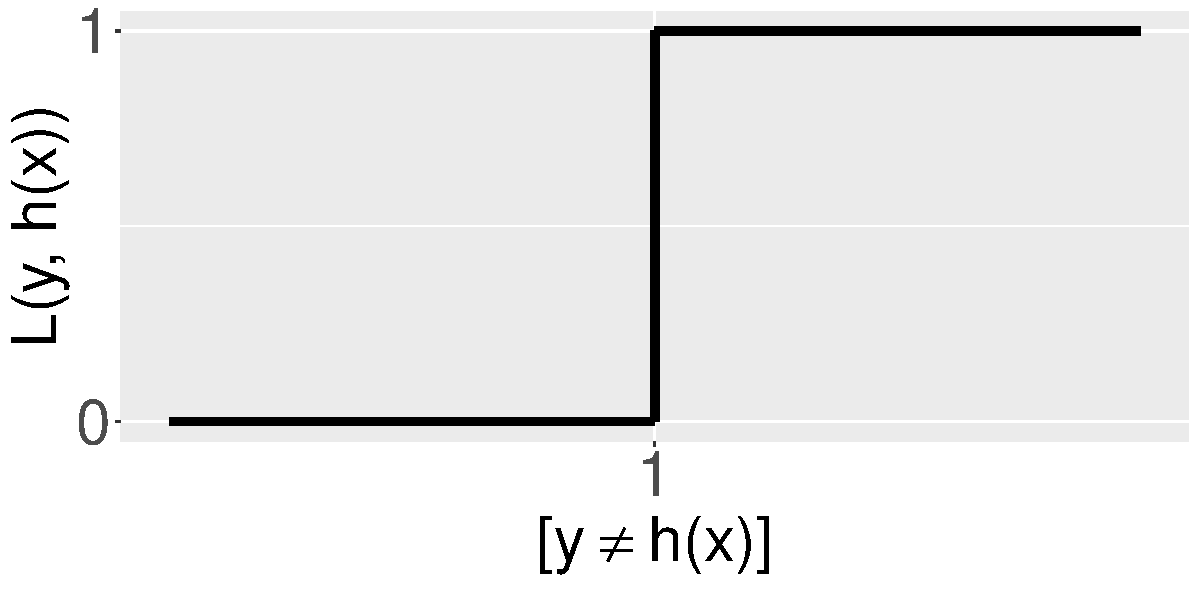
\includegraphics[width=0.8\textwidth]{figure/zero-one-loss}
\end{minipage}

\lz

\begin{itemize}
  \item Problem: 0-1 loss is not differentiable (not continuous even). \\
  $\rightarrow$ This is why we use \textbf{binomial} loss as inner loss 
  instead.
  \item For evaluation, differentiability is not required, so evaluation on 
  \textbf{MCE} is feasible. 
\end{itemize}

\normalsize

\end{vbframe}

% ------------------------------------------------------------------------------

\endlecture
\end{document}
